%%%%%%%%%%%%%%%教案头%%%%%%%%%%%%%%%%%%%%%%%%%%%%%%%
\mode <article>{

\begin{longtable}{|m{20mm}|m{20mm}|m{20mm}|m{20mm}|m{20mm}|m{28mm}|}
\caption*{\huge 教案头}\\
\hline
\endfirsthead
\multicolumn{6}{l}{(续表)}\\
\hline
\endhead
\hline
\multicolumn{6}{l}{\itshape 接下一页表格.......}\\ [2ex]
\endfoot
\hline
\endlastfoot
\centering{授课单元}&\multicolumn{3}{m{60mm}|}{\centering 引论}&\centering{授课日期}&2014年03月14日 \\
\hline
\centering 授课地点 & \multicolumn{3}{m{60mm}|}{B6-204}&\centering 授课学时 & 2 \\
\hline
& \multicolumn{2}{m{40mm}|}{能力目标} & \multicolumn{2}{m{40mm}|}{知识目标}&素质目标 \\
\cline{2-6}
\centering 教学目标&\multicolumn{2}{m{40mm}|}{\begin{enumerate}
\item 能够分析控制系统的类型
\end{enumerate}} &\multicolumn{2}{m{40mm}|}{\begin{enumerate}
\item 掌握计算机控制系统的概念
\item 掌握控制系统的分类
\item 了解计算机控制系统的研究内容
\item 掌握计算机控制系统的基本要求
\end{enumerate}} & {\qquad}\\
\hline
\centering 能力训练任务或案例 &\multicolumn{5}{m{108mm}|}{\begin{enumerate}
\item 电吹风的控制电路图
\item 电饭堡的控制电路图
\end{enumerate}}\\
\hline
\centering 教学重点 & \multicolumn{5}{m{108mm}|}{计算机控制系统的基本要求}\\
\hline
\centering 教学难点与解决办法 &\multicolumn{5}{m{108mm}|}{无}\\
\hline
\centering 德育内容 &\multicolumn{5}{m{108mm}|}{无}\\
\hline
 &教材 & \multicolumn{4}{l|}{计算机控制原理与应用}\\
\cline{2-6}& 教学资源 &\multicolumn{4}{m{88mm}|}{PPT}\\
\cline{2-6}\centering 使用的教学材料& 主要教学仪器设备和工具等 &\multicolumn{4}{m{88mm}|}{投影机、MATLAB}\\
\cline{2-6}& 主要耗材 &\multicolumn{4}{m{88mm}|}{\qquad}\\
\hline
\centering 教学模式 &\multicolumn{2}{l|}{知识讲授}&\centering 教学手段 &\multicolumn{2}{l|}{多媒体教学}\\
\hline
\centering 学生成果与过程考核方式 &\multicolumn{5}{m{108mm}|}{无}
\end{longtable}
\clearpage

%%%%%%%%%%%%%%%教学实施过程%%%%%%%%%%%%%%%%%%%%%%%%%%%%
\begin{landscape}

\begin{longtable}{|m{10mm}|m{50mm}|m{50mm}|m{50mm}|m{15mm}|}
\caption*{\huge 教学组织与实施}\\
\hline
\endfirsthead
\multicolumn{5}{l}{\small 接上页}\\
\hline
\multicolumn{1}{|c|}{步骤}&\multicolumn{1}{c|}{教学内容}&\multicolumn{1}{c|}{教师活动}&\multicolumn{1}{c|}{学生活动}&\multicolumn{1}{c|}{时间}\\
\hline
\endhead

\multicolumn{5}{r}{\small 接下页}\\
\endfoot
\hline
\endlastfoot
\multicolumn{1}{|c|}{步骤}&\multicolumn{1}{c|}{教学内容}&\multicolumn{1}{c|}{教师活动}&\multicolumn{1}{c|}{学生活动}&\multicolumn{1}{c|}{时间}\\\hline
引入&\begin{enumerate}
\item 计算机控制的概念
\end{enumerate} &\begin{enumerate}
\item 播放与计算机控制有关的视频
\item 提问:从视频中你能够看出什么?实现这些的关键是什么?
\end{enumerate} &\begin{enumerate}
\item 学生观看视频,思考教师提出的问题。
\end{enumerate} &10 \\\hline
讲解&控制系统的分类
\begin{enumerate}
\item 连续(模拟)控制系统
\item 离散(数字)控制系统
\end{enumerate} &\begin{enumerate}
\item 以电吹风的例子讲解开环连续控制系统
\item 以电饭堡的例子讲解闭环边续控制系统
\item 讲解开环数字控制系统
\item 讲解闭环数字控制系统
\end{enumerate} &\begin{enumerate}
\item 学生分析电吹风的控制
\item 学生分析电饭堡的控制
\item 学生倾听
\end{enumerate} &30 \\\hline
总结&小结本节课的内容
&总结控制系统的分类 &\begin{enumerate}
\item 学生记录总结内容
\item 学生倾听
\end{enumerate} &5 \\\hline
讲解&计算机控制系统的分类
\begin{enumerate}
\item 数据采集与处理系统
\item 直接数字控制系
\item 监督控制系统
\item 分级控制系统
\item 集散控制系统
\end{enumerate} &\begin{enumerate}
\item 讲解数据采集与处理系统
\item 讲解直接数字控制系统
\item 讲解监督控制系统
\item 讲解分级控制系统
\item 讲解集散控制系统
\end{enumerate} &\begin{enumerate}
\item 学生记录笔记
\item 学生倾听
\end{enumerate} &30 \\\hline
讲解&计算机控制系统的研究内容
\begin{enumerate}
\item 系统建模
\item 系统分析
\item 系统设计
\end{enumerate}
对计算机控制系统的基本要求
\begin{enumerate}
\item 系统必须是稳定的
\item 动态过程必须满足动态性能指标的要求
\item 系统必须满足稳态误差要求
\end{enumerate} &\begin{enumerate}
\item 讲解计算机控制系统的研究内容
\item 讲解对计算机控制系统的要求
\end{enumerate} &\begin{enumerate}
\item 学生记录笔记
\item 学生倾听
\end{enumerate} &10 \\\hline
\centering 本次课总结(评价)&总结本课程内容 &进行知识总结 &学生倾听 &5 \\\hline
\centering 学生学习笔记或工单等检查情况&\multicolumn{4}{m{165mm}|}{\quad}\\\hline
\centering 课后作业&\multicolumn{4}{m{165mm}|}{\begin{enumerate}
\item 对计算机控制系统的基本要求是什么?
\item 计算机按照功能可分为哪几种典型系统?
\item 典型的计算机集成制造系统有哪四个功能系统和哪两个支持系统?
\end{enumerate}}\\\hline
\centering 教学体会&\multicolumn{4}{m{165mm}|}{\begin{itemize}
\item 对学生的学习兴趣激发不足,需要优化第一次课设计
\end{itemize}}
\end{longtable}

\end{landscape}
\clearpage
%%%%%%%%%%%%%%%%%%%%板书设计%%%%%%%%%%%%%%%%%%%%%%%%%%
\lecture{计算机控制系统简介}{yinlun}
\begin{center}
{\huge 板书设计}
\end{center}
}

\mode<presentation>{ \section{引论}
 \subsection{计算机控制系统}}
\begin{frame}
\begin{block}{自动控制}
\begin{itemize}
\item 无人参与
\item 通过控制器或控制装置控制物理设备或装置
\item 实现期望控制规律,达到控制目标
\end{itemize}
\end{block}
\begin{block}{自动控制的优点}
\begin{itemize}
\item 改善劳条件,解决劳动力
\item 提高生产效率和产品质量
\item 节约能源,降低成本
\end{itemize}
\end{block}
\end{frame}
\begin{frame}[containsverbatim]{计算机控制系统}
\begin{definition}
计算机控制系统:

强调计算机作为控制系统的一个重要组成部分
\end{definition}
计算机控制系统着重强调:
\begin{itemize}
\item 控制系统中包含数字信号
\item 只在时间点上采集和处理数据
\end{itemize}
\mode<presentation>{\subsection{控制系统分类}}
\end{frame}
\begin{frame}[containsverbatim]{连续控制系统}
\begin{definition}
连续控制系统:

控制系统传递的信息为连续(模拟)信号
\end{definition}
\begin{figure}[htbp]
\begin{tikzpicture}[>=stealth]
\draw[->,line width=0.7mm](-1cm,0)--(1cm,0)node[midway,above]{x};
\draw[line width=0.7mm](1cm,-0.5cm)rectangle(2.5cm,0.5cm);
\draw[->,line width=0.7mm](2.5cm,0)--(4.5cm,0)node[midway,above]{y};
\draw(1.75cm,0)node{\tiny 系统};
\draw(0,0)node[below]{\tiny (输入)};
\draw(3.5cm,0)node[below]{\tiny (输出)};
\end{tikzpicture}
\end{figure}
\end{frame}
\begin{frame}{电吹风电路图}
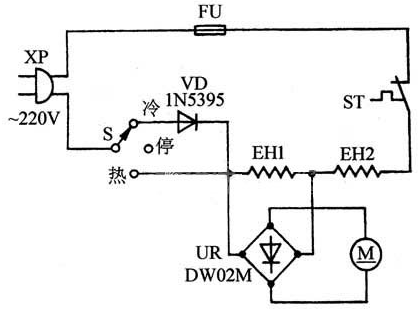
\includegraphics[scale=0.8]{diancuifeng.png}
\end{frame}
\begin{frame}[fragile]{开环控制系统}
\begin{tikzpicture}
[node distance=15mm,>=stealth,text height=1.5ex,text depth=.25ex]
\node(A)[nonterminal]{\tiny 控制器};
\node(B)[nonterminal,base right=of A]{\tiny 被控对象};
\draw[->](A)--(B)node[midway,above]{\tiny 控制变量};
\draw[<-](A.west)--++(-15mm,0)node[midway,above]{\tiny输入r(t)};
\draw[<-](B.north)--++(0,5mm)node[above]{\tiny 扰动 d(t)};
\draw[->](B.east)--++(15mm,0)node[midway,above]{\tiny 输出c(t)};
\end{tikzpicture}

\begin{block}{开环控制系统的特点}
\begin{itemize}
\item 只有顺序作用,没有反向联系。
\item 控制系统结构简单、经济。
\item 输入与输入是一一对应关系。
\item 干扰可使系统偏离期望值。
\end{itemize}
\end{block}
\end{frame}
\begin{frame}[containsverbatim]{闭环控制系统}
\begin{tikzpicture}
[node distance=10mm,>=stealth]
\node(start)[circleterminal,label=above left:\tiny +,label=below left:-]{};
\draw(start.south west)--(start.north east);
\draw(start.north west)--(start.south east);
\node(control)[nonterminal,base right=of start]{\tiny 控制器};
\node(obj)[nonterminal,base right=of control]{\tiny 被控对象};
\node(retu)[nonterminal,below=5mm of control]{\tiny 传感器};
\draw[<-](start.west)--++(-15mm,0)node[midway,above]{\tiny input r(t)};
\draw[->](start)--(control)node[midway,above]{\tiny e(t)};
\draw[->](control)--(obj)node[midway,above]{\tiny m(t)};
\draw(obj.east)--++(5mm,0)coordinate(a);
\filldraw(a)circle(2pt)node[above]{\tiny out c(t)};
\draw[->](a)--++(10mm,0);
\draw[->](a)|-(retu);
\draw[->](retu)-|(start)node[very near end,below right]{\tiny b(t)};
\draw[<-](obj.north)--++(0,5mm)node[above]{\tiny 扰动d(t)};
\end{tikzpicture}
\end{frame}
\begin{frame}{电饭煲电路图}
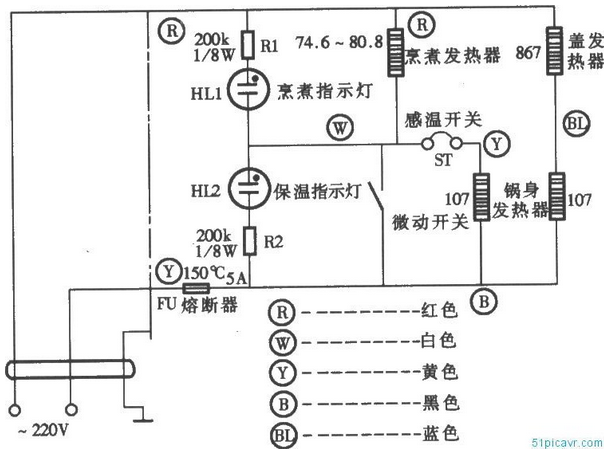
\includegraphics[scale=0.5]{dianfanbao.png}
\end{frame}
\begin{frame}[containsverbatim]{闭环控制系统}
\begin{block}{闭环控制系统的特点}
\begin{itemize}
\item 输出量能够自动跟踪给定量
\item 减小跟踪误差
\item 提高控制精度
\item 抑制撼动信息号的影响
\item 降低对前向通路中的元件精度要求
\end{itemize}
\end{block}
\end{frame}
\mode<presentation>{\subsection{离散控制系统}}
\begin{frame}[containsverbatim]{开环数字控制系统}
\begin{tikzpicture}
[node distance=10mm,>=stealth]
\node(ADC)[nonterminal,label=above:\tiny (接口)]{\tiny ADC};
\draw[<-](ADC.west)--++(-15mm,0)node[midway,label=above:\tiny input r(t),label=below:\tiny 设定值]{};
\node(control)[nonterminal,right= of ADC,label=above:\tiny (计算机)]{\tiny 控制算法};
\draw[->](ADC.east)--(control.west)node[midway,above]{\tiny r(kT)};
\node(DAC)[nonterminal,right=of control,label=above:\tiny (接口)]{\tiny DAC};
\draw[->](control.east)--(DAC.west)node[midway,above]{\tiny m(kT)};
\node(obj)[nonterminal,right=of DAC]{\tiny 被控对象};
\draw[->](DAC.east)--(obj.west)node[midway,above]{\tiny m(t)};
\draw[->](obj.east)--++(10mm,0)node[midway,above]{\tiny out c(t)};
\draw[<-](obj.north)--++(0,5mm)node[above]{\tiny 扰动d(t)};
\end{tikzpicture}
\end{frame}
\begin{frame}[containsverbatim]{闭环数字控制系统}
\begin{tikzpicture}
[node distance=10mm,>=stealth]
\node(ADD)[circleterminal,label=above left:\tiny +,label=below left:-]{};
\draw[<-](ADD.west)--++(-15mm,0)node[midway,label=above:\tiny r(kT)]{};
\draw(ADD.south west)--(ADD.north east);
\draw(ADD.north west)--(ADD.south east);
\node(control)[nonterminal,right= of ADD,label=above:\tiny (计算机)]{\tiny 控制算法};
\draw[->](ADC.east)--(control.west)node[midway,above]{\tiny e(kT)};
\node(DAC)[nonterminal,right=of control,label=above:\tiny (接口)]{\tiny DAC};
\draw[->](control.east)--(DAC.west)node[midway,above]{\tiny m(kT)};
\node(obj)[nonterminal,right=of DAC]{\tiny 被控对象};
\draw[->](DAC.east)--(obj.west)node[midway,above]{\tiny m(t)};
\draw[->](obj.east)--++(5mm,0)coordinate(a)node[above]{\tiny out c(t)}--++(10mm,0);
\filldraw(a)circle(2pt);
\draw[<-](obj.north)--++(0,5mm)node[above]{\tiny 扰动d(t)};
\node(ADC)[nonterminal,below=5mm of DAC,label=below:\tiny(接口)]{\tiny ADC};
\draw[->](a)|-(ADC);
\draw[->](ADC.west)-|(ADD.south)node[ near start,above]{\tiny c(kT)};
\end{tikzpicture}
\end{frame}
\mode<presentation>{\subsection{计算控制系统分类}}
\begin{frame}[containsverbatim]{数据采集与处理系统}
\begin{tikzpicture}
[node distance=5mm,>=stealth]
\node(obj)[nonterminal,text width=3mm,text depth=10em,text height=2em]{\tiny 过程或被 控制对象};
\node(caiyang)[nonterminal,below left= of obj.north west]{\tiny 采\qquad 样};
\draw[<-](caiyang.east)--(caiyang.east-|obj.west);
\node(celiang1)[nonterminal,below=of caiyang]{\tiny 测\qquad 量};
\draw[<-](celiang1.east)--(celiang1.east-|obj.west);
\node(celiang2)[nonterminal,below=of celiang1]{\tiny 测\qquad 量};
\draw[<-](celiang2.east)--(celiang2.east-|obj.west);
\node(chixing)[nonterminal,below=of celiang2]{\tiny 执行机构};
\draw[->](chixing.north east)--(chixing.north east-|obj.west);
\draw[->](chixing.south east)--(chixing.south east-|obj.west);
\node(ADC)[nonterminal,left=of caiyang]{\tiny ADC};
\draw[<-](ADC)--(caiyang);
\node(computer)[nonterminal,text width=2mm,text depth=6em,text height=2em,left=20mm of celiang1]{\tiny  计算机 };
\draw[->](ADC)--(ADC-|computer.east);
\draw[->](celiang2.west)--(celiang2.west-|computer.east);
\draw[->](celiang1.west)--(celiang1.west-|computer.east);
\node(record)[nonterminal,left = of computer]{\tiny 记录};
\draw[<-](record.east)--(record.east-|computer.west);
\node(disp)[nonterminal,above=of record]{\tiny 显示};
\draw[<-](disp.east)--(disp.east-|computer.west);
\node(alter)[nonterminal,below=of record]{\tiny 报警};
\draw[<-](alter.east)--(alter.east-|computer.west);
\node(man)[circleterminal,left =of record]{\tiny 人};
\draw[->](record.west)--++(-2.5mm,0)coordinate(B)--(man.east);
\filldraw(B)circle(2pt);
\draw(B)|-(disp);
\draw(B)|-(alter);
\draw[->](man)|-(chixing);
\end{tikzpicture}
\end{frame}
\begin{frame}[containsverbatim]{直接数字控制系统}
\begin{tikzpicture}
[node distance=5mm,>=stealth]
\node(value)[nonterminal]{\tiny 给定值};
\node(disp)[nonterminal,text width=5mm,below=of value]{\tiny 显示记录报警};
\node(oprat)[nonterminal,text width=2mm,above right=of disp.south east]{\tiny  操作控制台\qquad};
\draw[->](value.east)--(value.east-|oprat.west);
\draw[<-](disp.east)--(disp.east-|oprat.west);
\node(computer)[nonterminal,text width=2mm,right =of oprat,text height=2em,text depth=10em,align=center]{\tiny计算机};
\draw[->]($(oprat.north east)+(0,-4mm)$)coordinate(a1)--(a1-|computer.west);
\draw[<-]($(oprat.south east)+(0,4mm)$)coordinate(a2)--(a2-|computer.west);
\node(celiang2)[nonterminal,right=30mm of computer]{\tiny 测\quad 量};
\draw[->](celiang2.west)--(celiang2.west-|computer.east);
\node(celiang1)[nonterminal,above=of celiang2]{\tiny 测\quad量};
\draw[->](celiang1.west)--(celiang1.west-|computer.east);
\node(cuangan)[nonterminal,above=of celiang1]{\tiny 传感器};
\node(ADC)[nonterminal,left=10mm of cuangan]{\tiny ADC};
\draw[->](cuangan.west)--(ADC.east);
\draw[->](ADC.west)--(ADC.west-|computer.east);
\node(chixing1)[nonterminal,below=of celiang2]{\tiny 执行器};
\node(DAC)[nonterminal,left=10mm of chixing1]{\tiny DAC};
\draw[<-](chixing1.west)--(DAC.east);
\draw[<-](DAC.west)--(DAC.west-|computer.east);
\node(chixing2)[nonterminal,below=of chixing1]{\tiny 执行器};
\draw[<-](chixing2.west)--(chixing2.west-|computer.east);
\node(obj)[nonterminal,right=20mm of celiang2,text width=2mm,text depth=10em,text height=2em]{\tiny 过程或被控对象};
\draw[<-](cuangan.east)--(cuangan.east-|obj.west)node[midway,above]{\tiny (模拟量)};
\draw[<-](celiang1.east)--(celiang1.east-|obj.west)node[midway,above]{\tiny (数字量)};
\draw[<-](celiang2.east)--(celiang2.east-|obj.west)node[midway,above]{\tiny (开关量)};
\draw[->](chixing1.east)--(chixing1.east-|obj.west)node[midway,above]{\tiny (模拟量)};
\draw[->](chixing2.east)--(chixing2.east-|obj.west)node[midway,above]{\tiny (模拟量)};
\end{tikzpicture}
\end{frame}
\begin{frame}[containsverbatim]{监督控制系统}
\begin{tikzpicture}
[node distance=5mm,>=stealth]
\node(disp)[nonterminal,text width=5mm]{\tiny 显示记录报警};
\node(opera)[nonterminal,text width=5mm,below=of disp]{\tiny 操作控制台};
\node(computer)[nonterminal,text width=3mm,below right=of disp.north east,text depth=5em,text height=0.5em]{\tiny SCC 计算机};
\draw[<-](disp.east)--(disp.east-|computer.west);
\draw[->](opera.east)--(opera.east-|computer.west);
\node(ADC)[nonterminal,above right=of computer.east]{\tiny ADC};
\draw[->](ADC.west)--(ADC.west-|computer.east);
\node(DAC)[nonterminal,below right=of computer.east]{\tiny DAC};
\draw[<-](DAC.west)--(DAC.west-|computer.east);
\node(celiang)[nonterminal,right=10mm of ADC]{\tiny 测量装置};
\draw[<-](ADC.east)--(celiang.west);
\node(moni)[nonterminal,right=10mm of DAC]{\tiny 模拟控制器};
\draw[->](DAC.east)--(moni.west);
\draw[->]($(ADC.east)+(3mm,0)$)|-($(moni.west)+(0,2mm)$);
\node(obj)[nonterminal,text width=3mm,right=40mm of computer.east]{\tiny 过程或被控制对象};
\draw[<-](celiang.east)--(celiang.east-|obj.west);
\draw[->](moni.east)--(moni.east-|obj.west);
\end{tikzpicture}
\end{frame}
\begin{frame}[containsverbatim]{监督控制系统}
\begin{tikzpicture}
[node distance=5mm,>=stealth]
\node(disp)[nonterminal,text width=5mm]{\tiny 显示记录报警};
\node(opera)[nonterminal,text width=5mm,below=of disp]{\tiny 操作控制台};
\node(computer)[nonterminal,text width=3mm,below right=of disp.north east,text depth=5em,text height=3em]{\tiny SCC 计算机};
\draw[<-](disp.east)--(disp.east-|computer.west);
\draw[->](opera.east)--(opera.east-|computer.west);
\node(DDC)[nonterminal,text width=3mm,text depth=5em,right=of computer.east]{\tiny DDC 计算机};
\draw[->](computer.east)--(DDC.west);
\node(ADC)[nonterminal,above right=10mm of DDC.east]{\tiny 接口};
\draw[->](ADC.west)--(ADC.west-|DDC.east);
\draw[->]($(ADC.west)+(-3mm,0)$)|-($(computer.north east)+(0,-2mm)$);
\node(DAC)[nonterminal,below right=10mm of DDC.east]{\tiny 接口};
\draw[<-](DAC.west)--(DAC.west-|DDC.east);
\node(celiang)[nonterminal,right= of ADC]{\tiny 测量装置};
\draw[<-](ADC.east)--(celiang.west);
\node(moni)[nonterminal,right= of DAC]{\tiny 执行器};
\draw[->](DAC.east)--(moni.west);
\node(obj)[nonterminal,text width=3mm,right=50mm of computer.east]{\tiny 过程或被控制对象};
\draw[<-](celiang.east)--(celiang.east-|obj.west);
\draw[->](moni.east)--(moni.east-|obj.west);
\end{tikzpicture}
\end{frame}
\begin{frame}[containsverbatim]{分级控制系统}
\begin{tikzpicture}
[scale=0.6,node distance=1mm,>=stealth]
\node(a1)[nonterminal]{\tiny 市场信息};
\draw[->](a1.east)--($(a1.east)+(5mm,0)$)coordinate(b1);
\node(a2)[nonterminal,below= of a1]{\tiny 计划调度};
\draw[->](a2.east)--($(a2.east)+(5mm,0)$);
\node(a3)[nonterminal,below= of a2]{\tiny 库房数据};
\draw[->](a3.east)--($(a3.east)+(5mm,0)$);
\node(a4)[nonterminal,below= of a3]{\tiny 订货销售};
\draw[->](a4.east)--($(a4.east)+(5mm,0)$);
\node(a5)[nonterminal,below= of a4]{\tiny 其它信息};
\draw[->](a5.east)--($(a5.east)+(5mm,0)$);
\draw[->]($(a5.south east)+(0,-3mm)$)node[left]{\tiny \vdots\qquad}--++(5mm,0)coordinate(b2);
\draw(b1)--(b2);
\node(a6)[nonterminal,below=5mm of a5]{\tiny 上送数据};
\draw[->](a6.east)--++(5mm,0)coordinate(b3);
\node(a7)[nonterminal,below= of a6]{\tiny 决策信息};
\draw[->](a7.east)--++(5mm,0);
\node(a8)[nonterminal,below= of a7]{\tiny 其它工厂};
\draw[->](a8.east)--++(5mm,0);
\draw[->]($(a8.south east)+(0,-3mm)$)node[left]{\tiny \vdots\qquad}--++(5mm,0)coordinate(b4);
\draw(b3)--(b4);
\draw($(b1)!.5!(b2)$)--++(5mm,0)coordinate(c1);
\draw($(b3)!.5!(b4)$)--++(5mm,0)coordinate(c2);
\node(temp)at($(b1)!.5!(b4)$){};
\node(computer1)[nonterminal,right=6mm of temp ,text width=3mm,label=above:\tiny (企业)]{\tiny 经营管理计算机};
\draw[->](c1)|-($(computer1.west)+(0,4mm)$);
\draw[->](c2)|-($(computer1.west)+(0,-4mm)$);
\node(computer2)[nonterminal,right=3mm of computer1 ,text width=3mm,label=above:\tiny (工厂)]{\tiny 集中监控计算机};
\draw[<->](computer1.east)--(computer2.west);
\node(temp1)at($(computer2.north east)!.5!(computer2.east)$){};
\node(temp2)at($(computer2.south east)!.5!(computer2.east)$){};
\node(SCC1)[nonterminal,right=3mm of temp1,text width=5mm]{\tiny SCC 计算机};
\draw[<->](SCC1.west)--(SCC1.west-|computer2.east);
\node(SCC2)[nonterminal,right=3mm of temp2,text width=5mm]{\tiny SCC 计算机};
\draw[<->](SCC2.west)--(SCC2.west-|computer2.east);
\node(temp3)at($(SCC1.north east)!.5!(SCC1.east)$){};
\node(temp4)at($(SCC1.south east)!.5!(SCC1.east)$){};
\node(DDC1)[nonterminal,right=3mm of temp3]{\tiny DDC 计算机};
\draw[<->](DDC1.west)--(DDC1.west-|SCC1.east);
\node(celiang1)[nonterminal,right=5mm of temp4]{\tiny 测\qquad量};
\draw[<->](celiang1.west)--(celiang1.west-|SCC1.east);
\node(obj1)[nonterminal,right=24mm of SCC1,text width=5mm,text height=0.5em]{\tiny 被控对象};
\draw[<->](DDC1.east)--(DDC1.east-|obj1.west);
\draw[<->](celiang1.east)--(celiang1.east-|obj1.west);
\node(temp5)at($(SCC2.north east)!.5!(SCC2.east)$){};
\node(temp6)at($(SCC2.south east)!.5!(SCC2.east)$){};
\node(DDC2)[nonterminal,right=3mm of temp5,label=above:\vdots]{\tiny DDC 计算机};
\draw[<->](DDC2.west)--(DDC2.west-|SCC2.east);
\node(celiang2)[nonterminal,right=5mm of temp6]{\tiny 测\qquad量};
\draw[<->](celiang2.west)--(celiang2.west-|SCC2.east);
\node(obj2)[nonterminal,right=24mm of SCC2,text width=5mm,text height=0.5em]{\tiny 被控对象};
\draw[<->](DDC2.east)--(DDC2.east-|obj2.west);
\draw[<->](celiang2.east)--(celiang2.east-|obj2.west);
\end{tikzpicture}
\end{frame}
\begin{frame}[containsverbatim]{集散控制系统}
\begin{tikzpicture}
[node distance=10mm,>=stealth]
\node(opera)[nonterminal]{\tiny 操作站};
\node(con)[nonterminal,below=of opera,text width= 7mm]{\tiny 监控计算机};
\node(temp)at($(opera.north east)!.5!(con.south east)$){};
\node(tongdao)[double arrow,draw,right=of temp, shape border rotate=90,text width=2mm]{\tiny 高速数据通道};
\draw[->]($(opera.east)+(0,1mm)$)coordinate(a1)--(a1-|tongdao.west);
\draw[<-]($(opera.east)+(0,-1mm)$)coordinate(a2)--(a2-|tongdao.west);
\draw[->]($(con.east)+(0,1mm)$)coordinate(a3)--(a3-|tongdao.west);
\draw[<-]($(con.east)+(0,-1mm)$)coordinate(a4)--(a4-|tongdao.west);
\node(base1)[nonterminal,right=30mm of opera]{\tiny 基本控制器};
\node(base2)[nonterminal,right=30mm of con,label=above:\vdots]{\tiny 基本控制器};
\draw[<-]($(base1.west)+(0,1mm)$)coordinate(a5)--(a5-|tongdao.east);
\draw[->]($(base1.west)+(0,-1mm)$)coordinate(a6)--(a6-|tongdao.east);
\draw[<-]($(base2.west)+(0,1mm)$)coordinate(a7)--(a7-|tongdao.east);
\draw[->]($(base2.west)+(0,-1mm)$)coordinate(a8)--(a8-|tongdao.east);
\node(obj1)[nonterminal,text width=10mm,right= of base1]{\tiny 过程或控制对象};
\node(obj2)[nonterminal,text width=10mm,right= of base2]{\tiny 过程或控制对象};
\draw[<-]($(obj1.west)+(0,1mm)$)coordinate(a9)--(a9-|base1.east);
\draw[->]($(obj1.west)+(0,-1mm)$)coordinate(a10)--(a10-|base1.east);
\draw[<-]($(obj2.west)+(0,1mm)$)coordinate(a11)--(a11-|base2.east);
\draw[->]($(obj2.west)+(0,-1mm)$)coordinate(a12)--(a12-|base2.east);
\end{tikzpicture}
\end{frame}
\mode<presentation>{\subsection{研究内容和基本要求}}
\begin{frame}[containsverbatim]{研究内容}
\begin{block}{}
\begin{itemize}
\item 系统建模
\item 系统分析
\item 系统设计
\end{itemize}
\end{block}
\end{frame}
\begin{frame}[containsverbatim]{基本要求}
\begin{block}{}
\begin{itemize}
\item 系统必须是稳定的
\item 动态过程必须满足动态性能指标的要求
\item 系统必须满足稳态误差的要求
\end{itemize}
\end{block}
\end{frame}
\endinput